\chapter{Seiten}

\section{Home}

Die Startseite des ACPs gibt eine allgemeine Schnellerklärung über alle Seiten des ACPs und ist die erste Seite auf der man nach der Anmeldung landet. Neben den allgemeinen Erklärungen stehen auf der Startseite Statistiken und Systeminformationen wie CPU-Auslastung, Laufzeit des Servers, RAM-Nutzung usw.

\begin{figure}[ht]
    \centering
    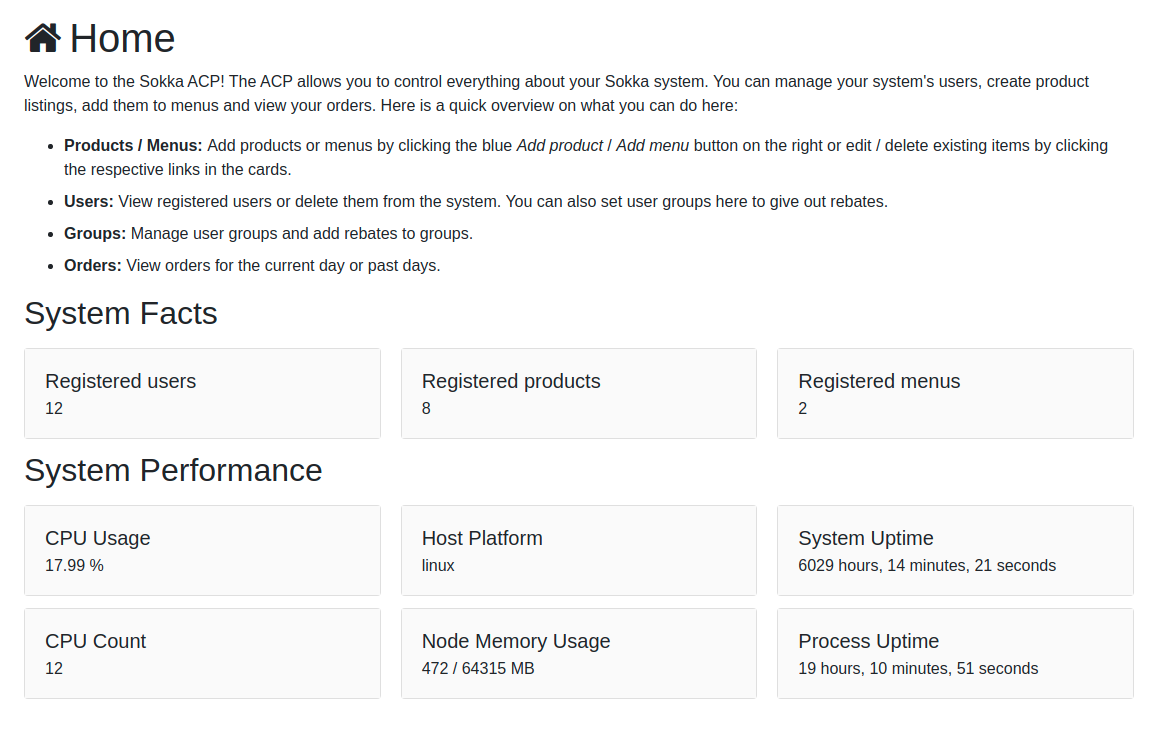
\includegraphics[width=0.8\textwidth]{images/ACP/home.png}
    \caption{Die Startseite des Sokka-ACPs}
\end{figure}

Die Informationen unter \textbf{System Facts} und \textbf{System Performance} aktualisieren sich alle fünf Sekunden automatisch.

\section{Products}

Die Produktseite erlaubt es Produkte im Sokka-System hinzuzufügen, zu bearbeiten und zu löschen.

\begin{figure}[ht]
    \centering
    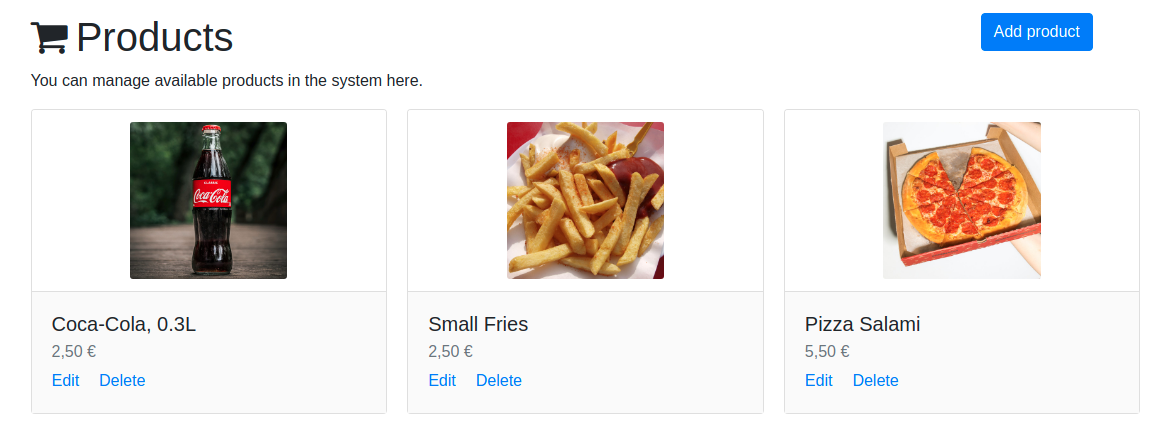
\includegraphics[width=0.8\textwidth]{images/ACP/products.png}
    \caption{Die Produkteseite des Sokka-ACPs}
\end{figure}

\section{Menus}

\begin{figure}[ht]
    \centering
    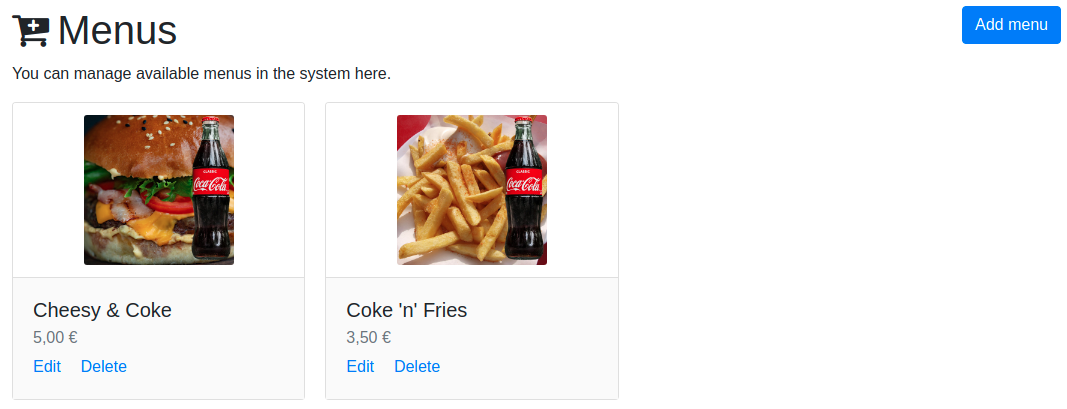
\includegraphics[width=0.8\textwidth]{images/ACP/menus.png}
    \caption{Die Menüsseite des Sokka-ACPs}
\end{figure}

\section{Users}

\begin{figure}[ht]
    \centering
    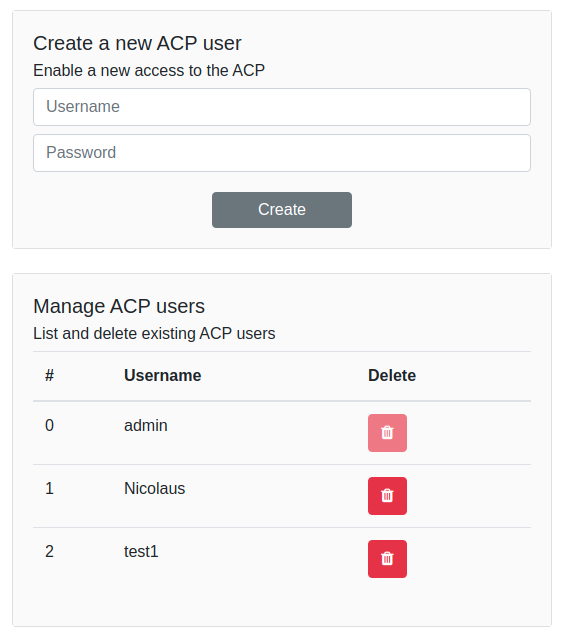
\includegraphics[width=0.8\textwidth]{images/ACP/users.png}
    \caption{Die Nutzerseite des Sokka-ACPs}
\end{figure}

\section{Groups}

\begin{figure}[ht]
    \centering
    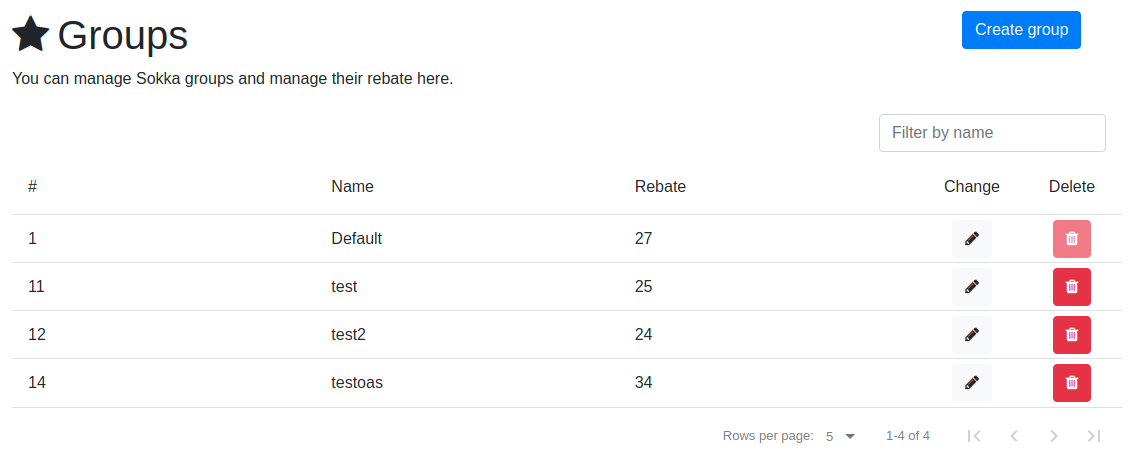
\includegraphics[width=0.8\textwidth]{images/ACP/groups.png}
    \caption{Die Gruppenseite des Sokka-ACPs}
\end{figure}

\section{Orders}

\begin{figure}[ht]
    \centering
    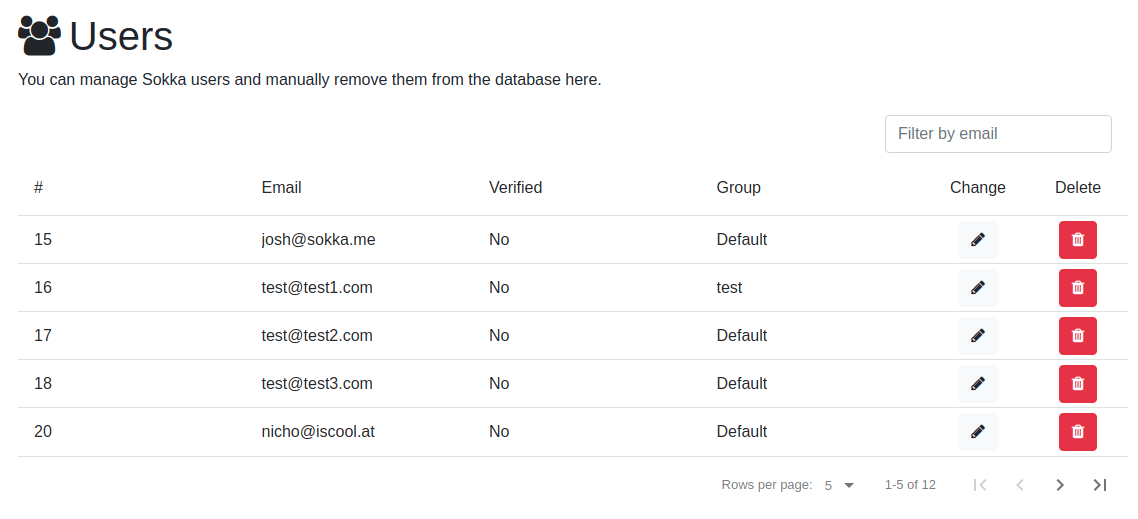
\includegraphics[width=0.8\textwidth]{images/ACP/users-page.png}
    \caption{Die Bestellungsseite des Sokka-ACPs}
\end{figure}

\section{Konfiguration}

\begin{figure}[ht]
    \centering
    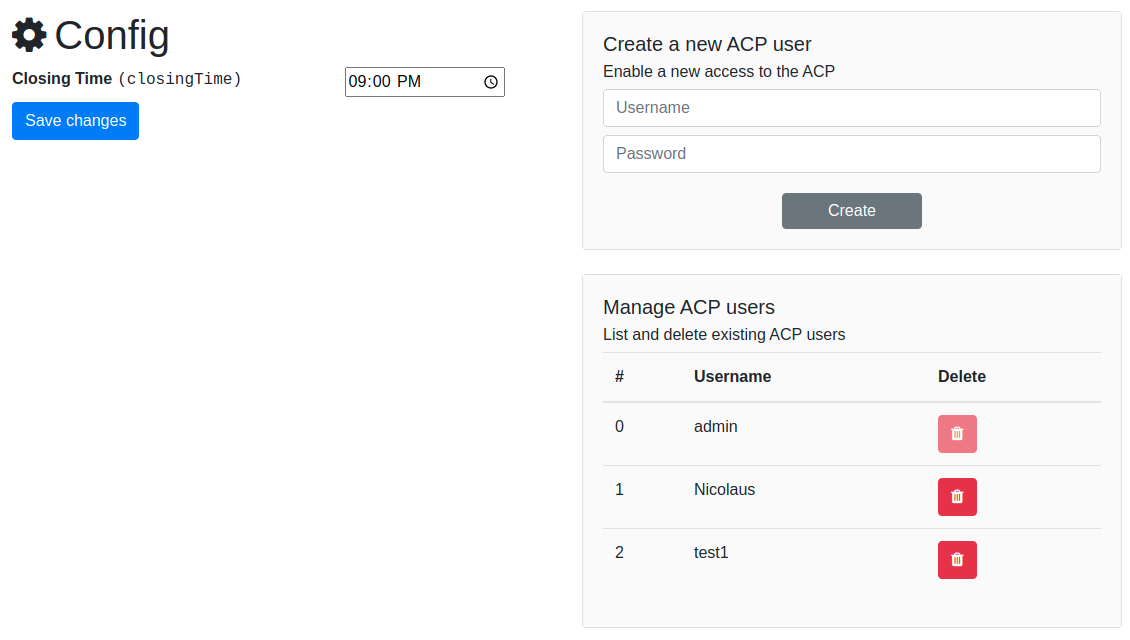
\includegraphics[width=0.8\textwidth]{images/ACP/config.png}
    \caption{Die Konfigurationsseite des Sokka-ACPs}
\end{figure}